\section{Zielsetzung}
In diesem Versuch soll die Funktionsweise eines Lock-In-Verstärkers untersucht werden.

\section{Theorie}
Der Lock-In-Verstärker wird meist für Messungen mit stark verrauschten Signalen benötigt, hierzu ist es notwendig
die zu messende Referenzfrequenz $\omega_0$ zu kennen.

\begin{figure}
  \centering
  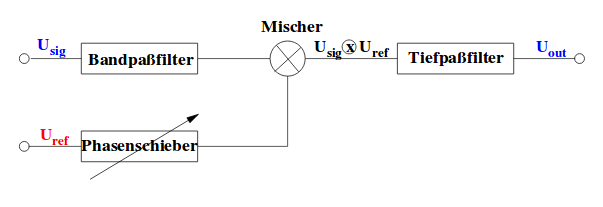
\includegraphics[scale = 0.6]{Aufbau.png}
  \caption{Schematischer Aufbau eines Lock-In-Verstärkers}
  \label{Aufbau}
\end{figure}

In Abbildung \ref{Aufbau} ist der Aufbau eines Lock-In-Verstärkers schematisch dargestellt. Das zu messende,
verrauschte Signal $U_\symup{sig}$ wird zunächst durch einen Bandpass geführt, sodass alle Frequenzen mit $\omega<<\omega_0$
und $\omega_0<<\omega$ herausgefitert werden. Das gefilterte Signal wird daraufhin in dem sogenannten Mischer mit einem Referenzsignal
$U_\symup{ref}$ multipliziert, wobei die Phase $\phi$ des Referenzsignals $U_\symup{ref}$ durch einen Phasenschieber verändert werden kann.
Zuletzt werden durch einen Tiefpass alle Oberfrequenzen heraus gefiltert, um eine konstante, messbare Gleichspannung $U_0$ zu erhalten,
wobei $U_0 \propto U_{out}$. Der Tiefpass fungiert außerdem als Integrator über mehrere Perioden des Mischsignals $U_\symup{sig} \cdot U_\symup{ref}$.

Der Vorteil eines Lock-In-Verstärkers im Gegensatz zu einem einfachen Bandpass ist die höhere Güte, welche etwa 100mal größer ist als bei
einem Bandpass (100.000:1.000).

In diesem Versuch sind sowohl $U_\symup{sig}$ und $U_\symup{ref}$ als Sinusspannungen mit der gleichen Referenzfrequenz anzusehen.
Mit

\begin{align*}
  U_\symup{sig} &= A_\symup{sig} \sin{(\omega t)} \\
  U_\symup{ref} &= A_\symup{ref} \sin{(\omega t + \phi)}
\end{align*}

folgt direkt

\begin{equation*}
  U_\symup{sig} \cdot U_\symup{ref} = A_\symup{sig} A_\symup{ref} \sin{(\omega t)} \sin{(\omega t + \phi)} ,
\end{equation*}

durch Umformen ergibt sich

\begin{equation}
  U_\symup{sig} \cdot U_\symup{ref} = \frac{1}{2} A_\symup{sig} A_\symup{ref} ( \cos{(\phi)} - \cos{(2 \omega t + \phi)})
\end{equation}

Durch den eben genannten Tiefpass, werden alle Oberschwingungen herausgefiltert und es bleibt nur der Gleichstromanteil übrig, der
folgend gemessen wird

\begin{equation}
  U_\symup{sig} \cdot U_\symup{ref} = \frac{1}{2} A_\symup{sig} A_\symup{ref} \cos{(\phi)} \, .
\end{equation}

\section{Durchführung}

Zunächst wird festgestellt, welcher Ausgang des Funktionsgenerators eine konstante und welcher eine variable Sinusspannung liefert,
dazu wird der Funktionsgenerator direkt an das Oszilloskop angeschlossen.

\begin{figure}
  \centering
  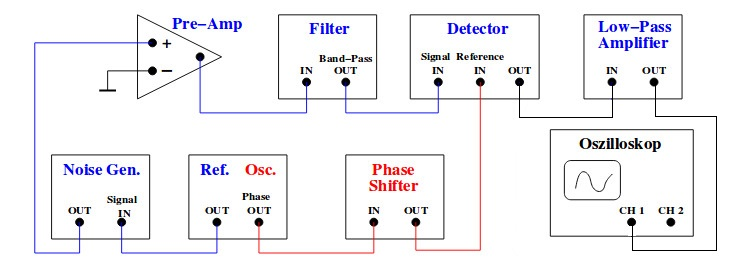
\includegraphics[scale = 0.6]{Aufbau2-korrigiert.jpeg}
  \caption{Versuchsaufbau 1.}
  \label{Aufbau1}
\end{figure}

Für den nächsten Teil des Versuchs wird das Experiment nach Abbildung \ref{Aufbau1} Schritt für Schritt aufgebaut, jedoch wird erst einmal der
Noise-Generator überbrückt. Es wird für das sinusförmige Ausgangssignal $U_\symup{sig}$ eine Frequenz von ca. \SI{1}{\kilo\hertz} und eine Amplitude
von \SI{10}{\milli\volt} eingestellt, indem der Funktionsgenerator direkt an das Oszilloskop angeschlossen wird und auf dem Bildschirm die
Frequenz und die Ampiltude überprüft werden kann. An dem anderen Ausgang des Funktionsgenerators wird eine sinusförmige Referenzspannung
$U_\symup{ref}$ mit gleicher Frequenz eingestellt. Folgend werden 5 Bilder von den Spannungsverläufen für verschiedene Phasen auf dem
Oszilloskop erstellt. Außerdem wird mit Hilfe des Oszilloskops die Ausgangsspannung in Abhängigkeit der Phasenverschiebung gemessen, hierzu
werden mindestens 10 Messwerte aufgenommen

Im nächsten Teil des Versuchs wird der Noise-Generator wieder mit in die Schaltung eingebunden. Es werden erneut 5 Bilder der Spannungsverläufe
für verschiedene Frequenzen auf dem Oszilloskop erstellt. Auch bei diesem Versuchsteil wird die Ausgangsspannung in Abhängigkeit der
Phasenverschiebung gemessen, wobei erneut mindestens 10 Messwerte aufgenommen werden.

\begin{figure}
  \centering
  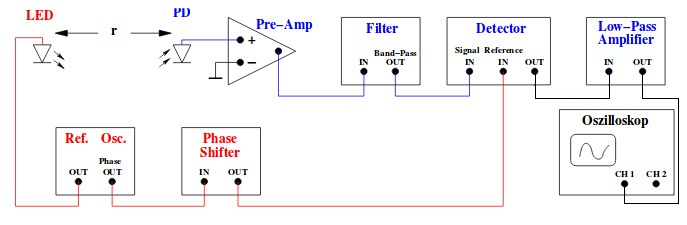
\includegraphics[scale = 0.7]{Aufbau1-korrigiert.jpeg}
  \caption{Versuchsaufbau 2.}
  \label{Aufbau2}
\end{figure}

Im letzten Teil des Versuchs wird eine Photodetektorschaltung nach Abbildung \ref{Aufbau2} aufgebaut. Die Leuchtdiode wird mit einer Rechteckspannung mit
einer Frequenz zwischen \SI{50}{\hertz} und \SI{500}{\hertz} betrieben. Das ausgestrahlte Licht wird mit einer Photodiode gemessen. Folgend wird die
Lichtintensität in Abhängigkeit des Abstandes gemessen. Hierzu werden mindestens 20 Messwerte und die maximale Weite des Lichtes $r_\symup{max}$
gemessen.
